\subsection{Escolha da aeronave}

Para escolha de uma aeronave que possa atender as necessidades impostas pelo projeto, deve considerar qual tipo de aplicação que a aeronave pode oferecer, escolhendo a melhor aeronavegável, que respeite todos os limites presentes no projeto. 

Considerando o fato de que o VANT (Veículo Aéreo Não-Tripulado) será utilizado para transporte de equipamento hospitalar, os aparelhos disponíveis para tal função são: VANT asa fixa e VANT asa rotativa (multirotors).

Os VANT’s de asa fixa, no caso, os aviões não tripulados, apesar de serem rápidos e possuírem um longo alcance de voo, para transporte de carga, exige tamanho da asa um pouco maior, pois a carga tem muito peso e para isso é preciso aumentar tanto o tamanho da asa, como o próprio avião. A aterrizagem é outro fator que dificulta pelo fato de que o aeromodelo exige um espaço aberto, com uma pista de pouso pelo menos do tamanho do aeromodelo. O que pode ser perigoso, pois o pouso será próximo de pessoas e um curto espaço para aterrissagem.

Os multirotors vêm aumentando no mercado nos últimos anos. Em termos mais simples, um multirotor usa várias hélices, em vez de uma única lâmina do rotor, como em um helicóptero tradicional, para fornecer elevação. Além disso, não há rotor de cauda, utilizada para fornecer controle de guinada e contrariar o torque posto para fora por dirigir o principal rotor em um helicóptero. Por serem simétricos, o controle de um multirotor é mais fácil e mais estável. O que permite uma decolagem e uma aterrissagem mais pratica e com menos espaço.
  
Os multirotors voam através da utilização de dois princípios básicos: elevação (lift) e torque.  Multirotors são verdadeiramente um grande exercício de física newtoniana: toda ação tem uma reação igual e oposta. Em um helicóptero tradicional, o rotor principal gira na mesma direção. Para manter o corpo de girar para o outro lado, um rotor de cauda é implementado de forma a colocar uma pressão constante sobre a cauda para manter o corpo estável. O multirotor usa hélices contra-rotação para manter o corpo estável, enquanto as hélices girarem \cite{audronis}.


\begin{figure}[h!]
    \centering
      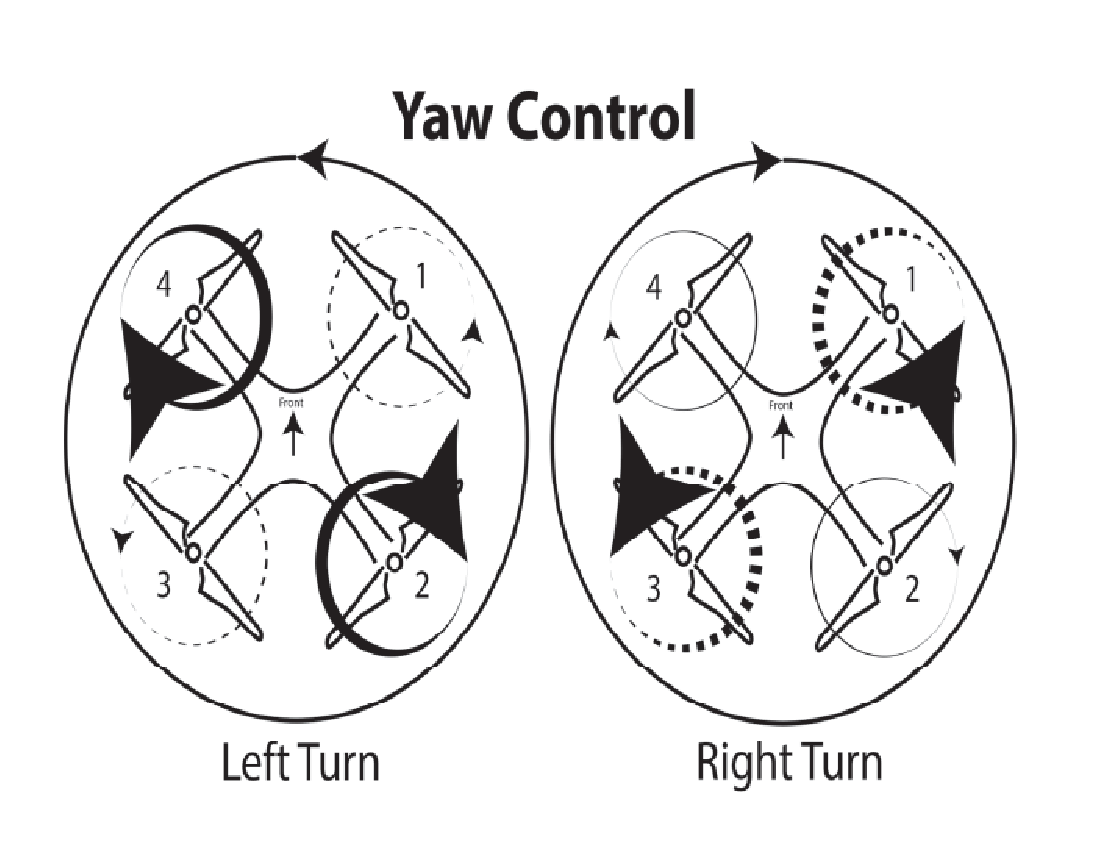
\includegraphics[keepaspectratio=true,scale=0.5]{figuras/gira.eps}
    \caption{Diagrama de gira para esquerda e para direita. Fonte \cite{audronis}}
    \label{fig:gira}
\end{figure}

Assim como um helicóptero tradicional, um multirotor se move para frente / trás e de lado para o outro pela inclinação. Inclinar o multirotor altera a direção do empuxo fornecido pelos rotores. Por exemplo, mergulhando o nariz e levantando a cauda, a direção na qual o fluxo de ar é empurrado é não só para baixo, mas também para a parte traseira do multirotor. Se toda a ação tem uma reação igual e opsta, empurrando o ar para a parte traseira do multirotor empurra para a frente o mesmo. Para fazer um mergulho de lado, a velocidade da hélice é reduzida, e para elevar um outro lado, a velocidade dos motores sobre que lado está aumentada.


\begin{figure}[h!]
    \centering
      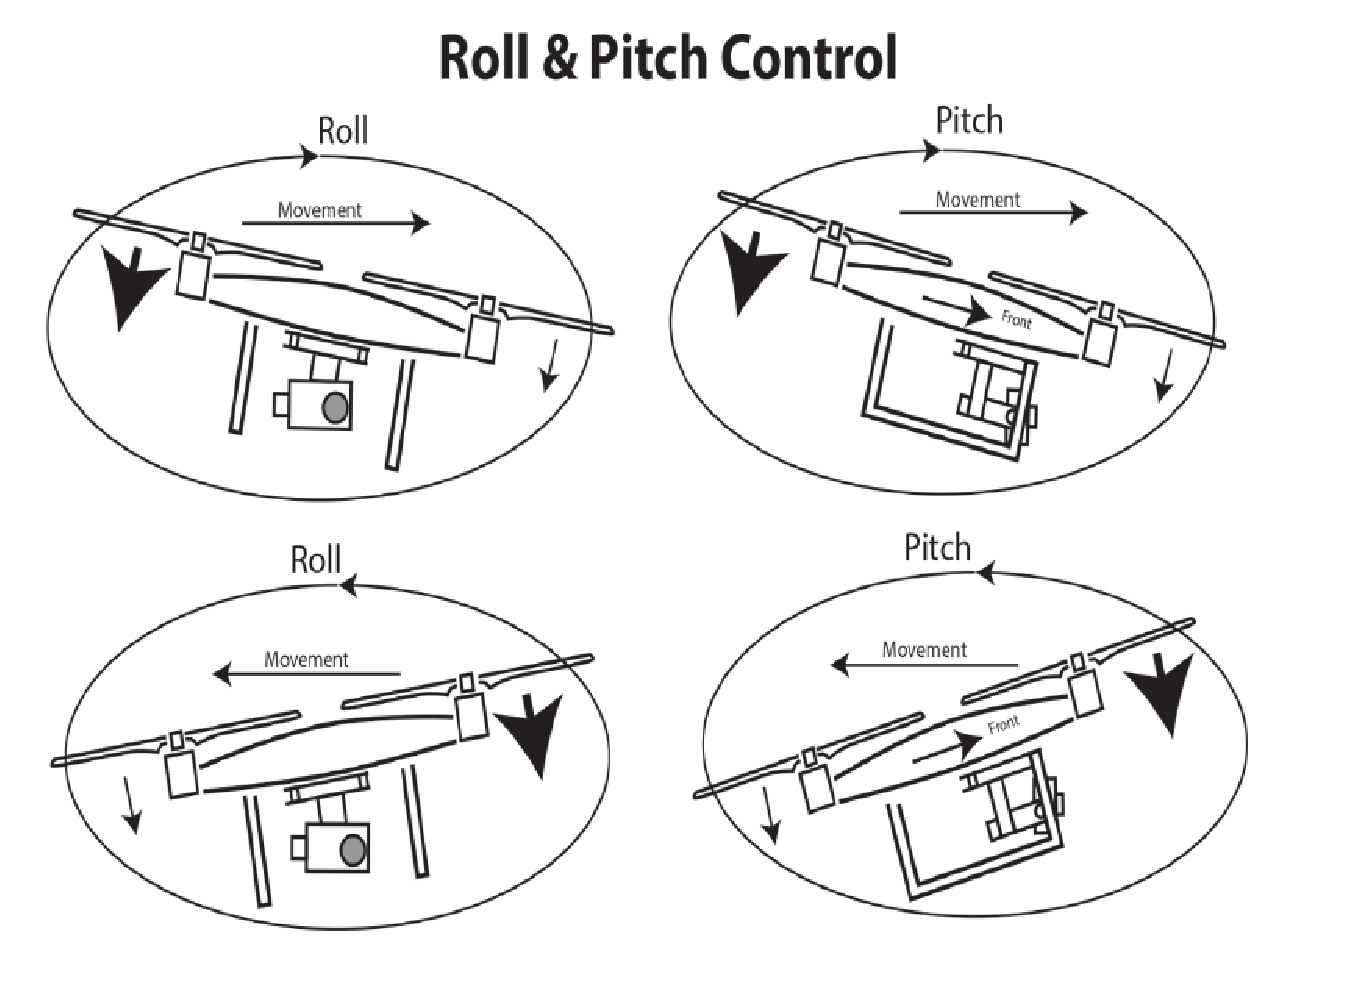
\includegraphics[keepaspectratio=true,scale=0.5]{figuras/guinada.eps}
    \caption{Diagrama de guinada e rolagem de um quadricóptero. Fonte \cite{audronis}}
    \label{fig:guinada}
\end{figure}

A desvantagem de utilizar os multirotors é a falta de aerodinâmica, tempo de voo reduzido e baixa eficiência dos motores. Contudo, para transporte de equipamento hospitalar, não exigirá um tamanho tão grande comparado a um aeromodelo.

\subsection{Especificação do VANT escolhido}

O multirotor escolhido para esse projeto é o de oito hélices, ou octocóptero. Embora oito rotores ofereçam mais estabilidade, também diminuem o tempo de voo, porque aumenta a pressão sobre baterias. De fato, o número de rotores em relação ao tempo de voo é exponencial e não linear. Mas como o projeto exige um peso maior, para melhor controle do VANT, o ideal seria o octocóptero. 

O motor escolhido é o motor Tarot 4114 High Power Brushless (sem escova) Motor, de alta rotação. Ele é usado pelo modelo US 1000 também octocóptero que é utilizado para filmagens. Ele possui capacidade de empuxo de até 2.5 kg. Este motor possui um rotor que é magnetizado por imãs permanentes. Motores de corrente contínua possuem vários benefícios em relação aos motores com escova, dentre algumas estão: melhor característica velocidade x torque, maiores eficiência, vida útil, taxa de velocidade e é mais silencioso \cite{nascimento}.

\begin{figure}[h!]
    \centering
      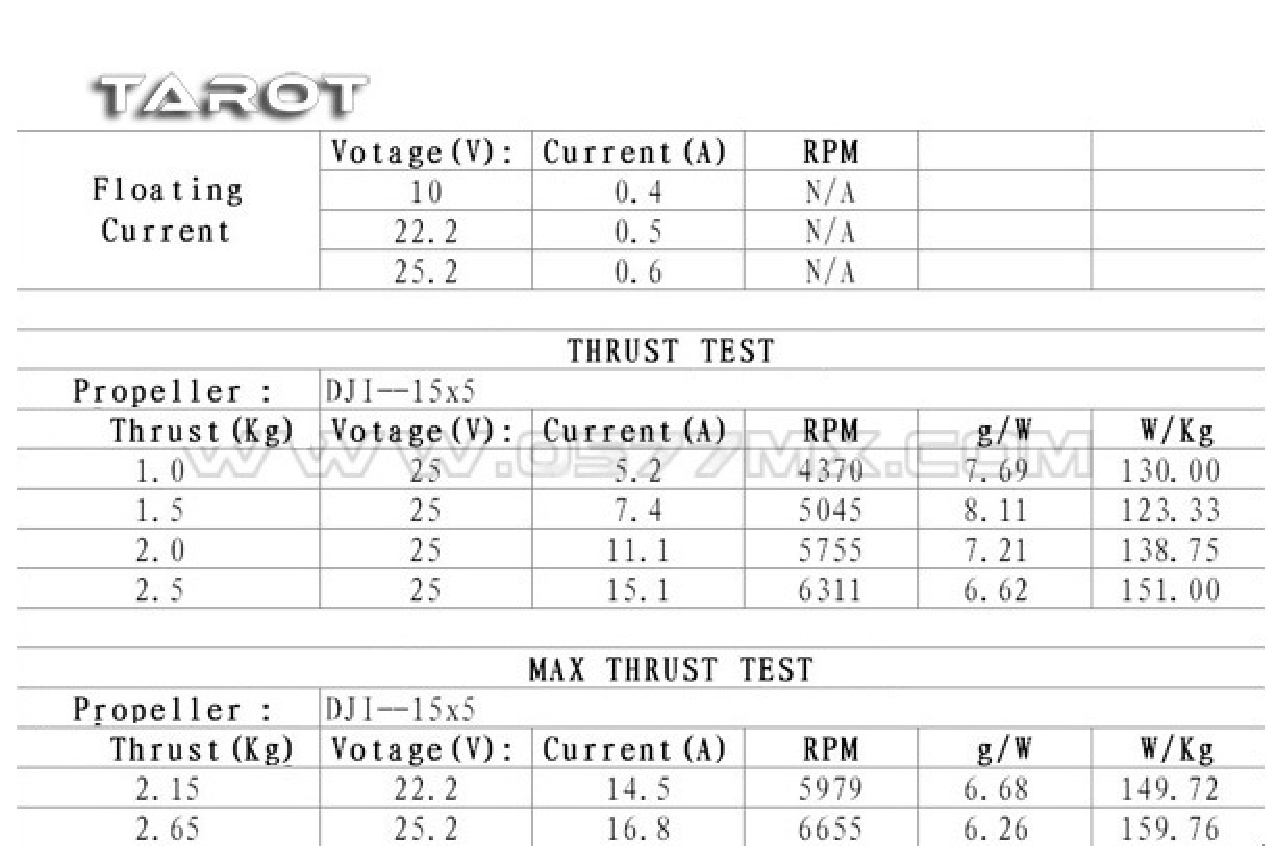
\includegraphics[keepaspectratio=true,scale=0.5]{figuras/tarot.eps}
    \caption{Quadro de relação de um motor 4114.}
    \label{fig:tarot}
\end{figure}

A hélice é um conjunto de pás com o mesmo centro, que ao ser girado causa uma propulsão na mesma direção. Utiliza-se duas pás por hélice. Quanto maior o passo da hélice, maior a velocidade alcançada pela aeronave e mais lenta é a resposta à manobras. Logo, o ideal é que o passo da hélice seja pequeno, pois é preferível uma melhor resposta à manobras, mesmo que seja preciso abrir mão de velocidade para tal \cite{VIOLATO}. A hélice escolhida é a 15x5 5.E Carbon Fiber Propellers L/H and R/H Rotation Suits DJI.

\begin{figure}[h!]
    \centering
      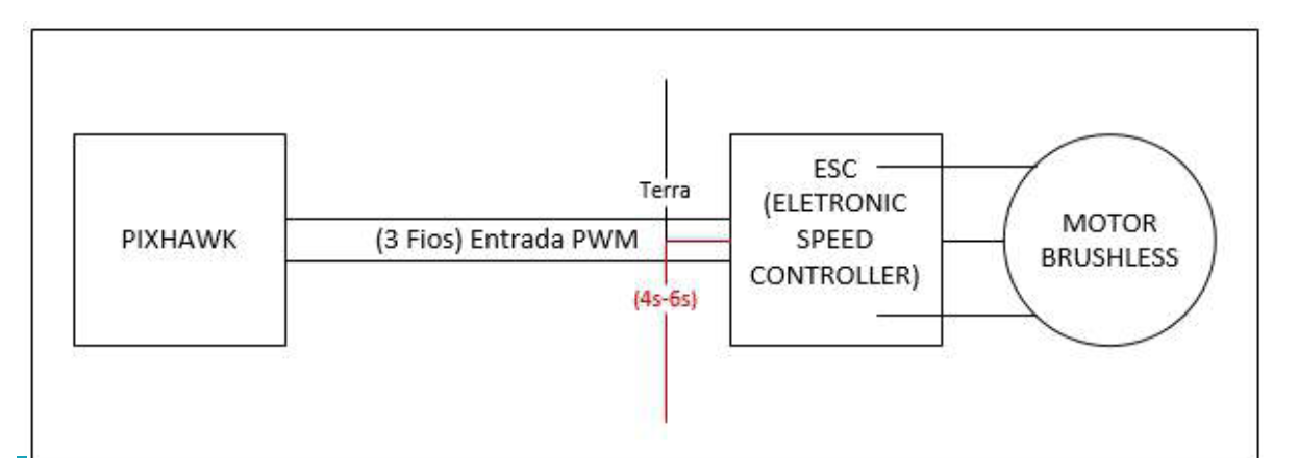
\includegraphics[keepaspectratio=true,scale=0.5]{figuras/elice.eps}
    \caption{Carbon Fiber Propellers L/H and R/H Rotation Suits DJI. Fonte: \cite{dji}}
    \label{fig:elice}
\end{figure}

\begin{figure}[h!]
    \centering
      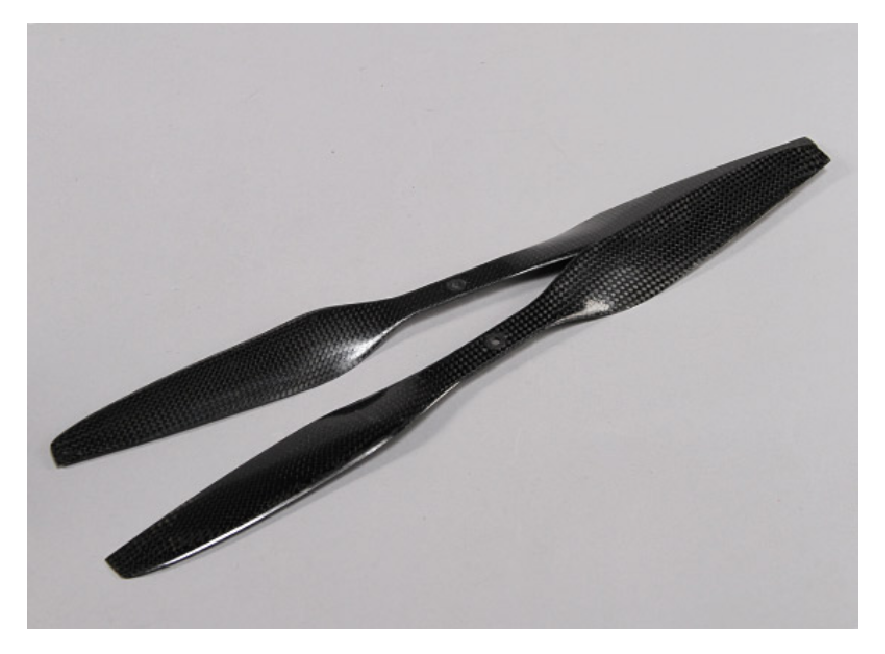
\includegraphics[keepaspectratio=true,scale=0.5]{figuras/diagramaEstru.eps}
    \caption{Esquemático de conexão e funcionamento do ESC. \cite{CASSEMIRO}}
    \label{fig:diagramaEstru}
\end{figure}

Os ESC (Eletronic speed control) é quem torna possível o voo. O ESC crava a tensão para ligar o motor e aliviá-lo de volta para mantê-los girando a uma velocidade baixa em um acelerador baixo. Além disso, como se aplica mais entrada do acelerador, o ESC acelera o motor de maneira uniforme.  Eles devem ser cuidadosamente equilibrados com o motor para dar energia suficiente para o motor e não queimar. No caso, deve ter um ESC individual para cada motor. 

\subsection{Escolha dos materiais}

A escolha de determinados materiais em projetos de engenharia depende de como os mesmos irão se comportar diante de um determinado esforço nas várias situações de aplicação.

Os componentes que farão parte do drone serão os motores de alto desempenho, as hélices, circuitos impressos e integrados e o corpo.
Esta delimitação de materiais que satisfazem as necessidades do drone foi feita levando em conta o tipo dos esforços que estarão presentes, por exemplo, na decolagem, aterrissagem e durante o tempo de voo. Para as hélices e para o motor foi escolhida a fibra de carbono e para o restante dos materiais a opção foi da fibra de vidro.

A justificativa para a escolha destes materiais foi baseada de acordo com o módulo de elasticidade, a ductilidade, o limite de resistência à tração e a tenacidade. 

Para que seja possível a visualização da comparação feita, as características citadas acima serão brevemente explicadas.


\begin{figure}[h!]
    \centering
      \includegraphics[keepaspectratio=true,scale=0.5]{figuras/grafico-tensao.eps}
    \caption{Gráfico Tensão-Deformação.}
    \label{fig:grafico-tensao}
\end{figure}

O módulo de elasticidade é a inclinação da região de comportamento elástico inicial da curva, ou seja, o coeficiente linear da reta antes de atingir a região de deslizamento de discordâncias.

% formula

A ductilidade é a medida do grau de deformação plástico que foi suportada até a fratura(F). Pode ser expressa quantitativamente como a porcentagem do alongamento percentual.

% formula

O limite de resistência à tração está caracterizado no gráfico como início da ruptura e indica o valor máximo de tensão que pode ser suportado por uma estrutura sob tração.
A tenacidade é definida como sendo a habilidade de um material absorver energia e se deformar plasticamente antes de fraturar.

\begin{figure}[h!]
    \centering
      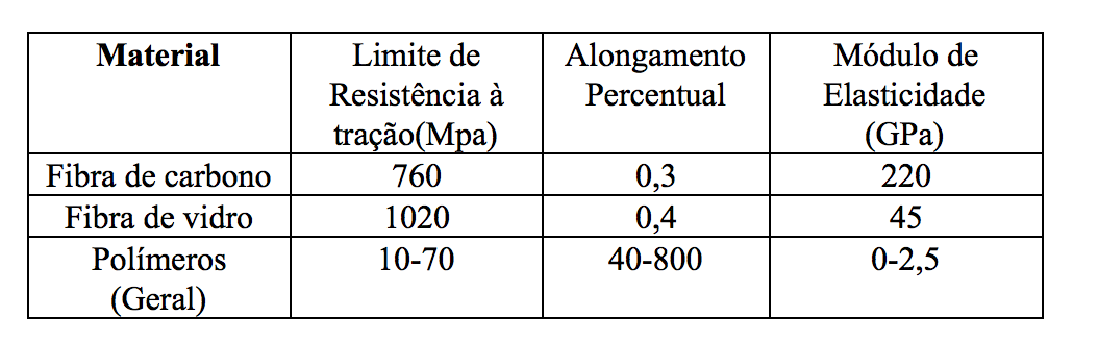
\includegraphics[keepaspectratio=true,scale=0.5]{figuras/graficoRelacao.eps}
    \caption{ Relação de materiais}
    \label{fig:graficoRelacao}
\end{figure}

Os materiais escolhidos, fibra de vidro e carbono, são determinados como materiais compósitos. As características destes incluem em pegar as melhores carcteristicas de variados materiais e junta-las para que se tenha um melhor desempenho no geral. 

Portanto, a escolha dos materiais do drone pode ser explicada de acordo com a tabela acima e com as explicações teóricas do que cada característica representa. 

Embora o alongamento percentual dos materiais poliméricos em geral seja muito maior do que os dos materiais ecolhidos para a aplicação do drone, esta característica é exibida no domínio plástico, ou seja, o material não se romperá mais perderá a qualidade devido a uma quantidade significativa de deformação.

Como conclusão do material a ser utilizado, é interessante partes da estrutura, como os braços, frame central, helices e trem de pouso, utilizando fibra de carbono. Partes como a carcaça e componentes eletrônicos, poderão ser utilizados polímeros em geral. 

\subsection{Construção do VANT}

Considerando a parte mais importante do projeto, o desfibrilador será acoplado no VANT, na qual suas medidas são utilizadas como referencia para modelagem do frame central. a modelagem dos  braços e hélices do drone, não serão necessários, devido eles serão utilizados do modelo de um VANT S1000.

Para inicio da construção do VANT, consideramos as medidas de um DEA (Desfibrilador externo automático) vendido no mercado, chamado HeartSine samaritan PAD SAM 300P. Com as seguintes  medidas:

\begin{figure}[h!]
    \centering
      \includegraphics[keepaspectratio=true,scale=0.5]{figuras/heart.eps}
    \caption{ HeartSine samaritan PAD SAM 300P}
    \label{fig:heart}
\end{figure}

O frame central projetado será baseado no frame central do S1000, porém adaptado ao desfibrilador e o reanimador. 

\begin{figure}[h!]
    \centering
      \includegraphics[keepaspectratio=true,scale=0.5]{figuras/framecentral.eps}
    \caption{ Frame central S1000}
    \label{fig:framecentral}
\end{figure}


Como as medidas, seguindo o manual, do frame central do S1000 é 337.5mm da ponta de um braço até outra, para o nosso projeto, será aumentado  200mm em relação ao centro, 100mm para um lado e 100mm par outro. Como mostra a figura a seguir:

\begin{figure}[h!]
    \centering
      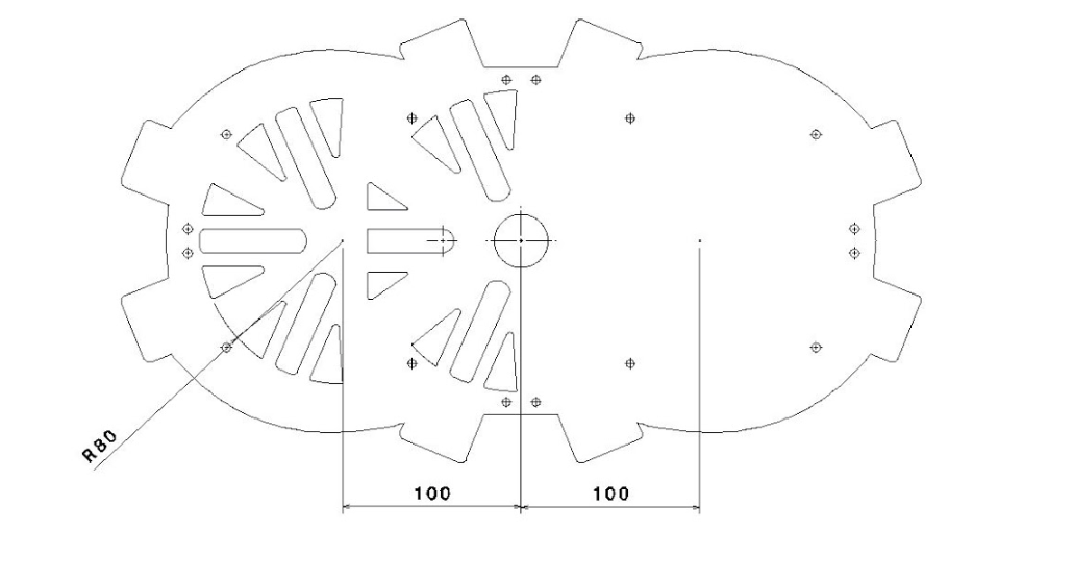
\includegraphics[keepaspectratio=true,scale=0.5]{figuras/drawing.eps}
    \caption{ Drawing Frame Central Superior}
    \label{fig:drawing}
\end{figure}

Como a figura acima mostra, as formas triangulares do lado esquerdo são “buracos” na qual tem como função deixar o frame mais leve, contudo, não perder sua utilidade em ser a base do VANT. O lado direito não possui esses espaços devido ser o local para alocar o desfibrilador. O lado esquerdo alocará a antena e até duas baterias , na qual serão presas por velcros, amarrados entre os “buracos” do frame. Também serão parafusadas os braços e a carcaça do VANT no mesmo.

\begin{figure}[h!]
    \centering
      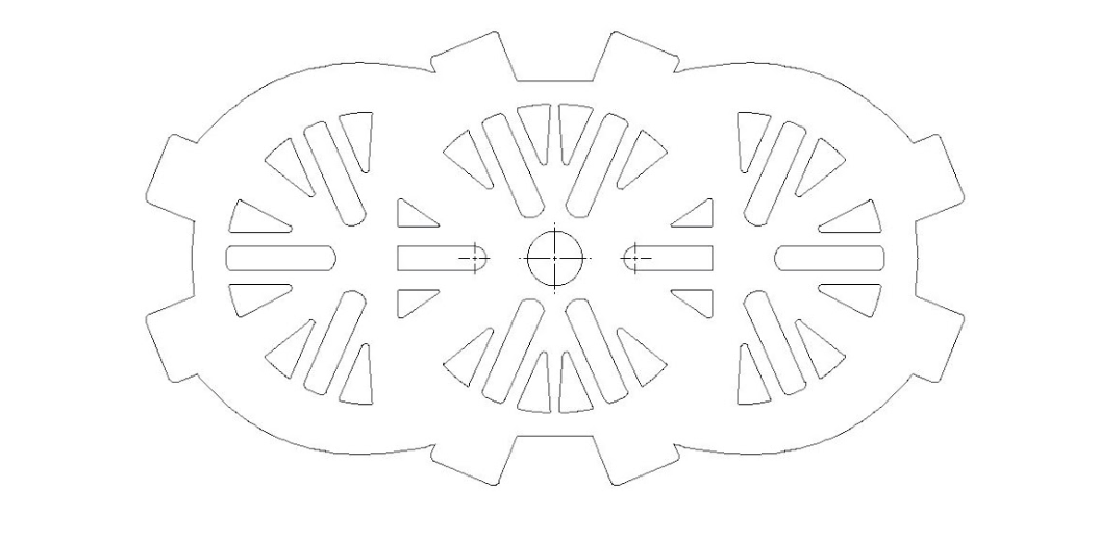
\includegraphics[keepaspectratio=true,scale=0.5]{figuras/drawinfinfo.eps}
    \caption{ Frame Central inferior}
    \label{fig:drawinfinfo}
\end{figure}

Já o frame inferior será parafusado o trem de pouso e o frame superior. Ambos os frames serão unidos como mostra a imagem 5, tendo um espaço de 42mm. O espaço entre os dois frames é destinado para alocar a parte dos controladores de voo , ESC e o conjunto dos fios.

\begin{figure}[h!]
    \centering
      \includegraphics[keepaspectratio=true,scale=0.5]{figuras/catia1.eps}
    \caption{Desenvolvimento do VANT no CATIA}
    \label{fig:catia1}
\end{figure}

Por meio da plataforma CATIA, foi possível idealizar o projeto EmerVANT, em escala real. Para visualizar de melhor forma, utilizou-se o KeyShot, na qual ele renderiza VANT.

\begin{figure}[h!]
    \centering
      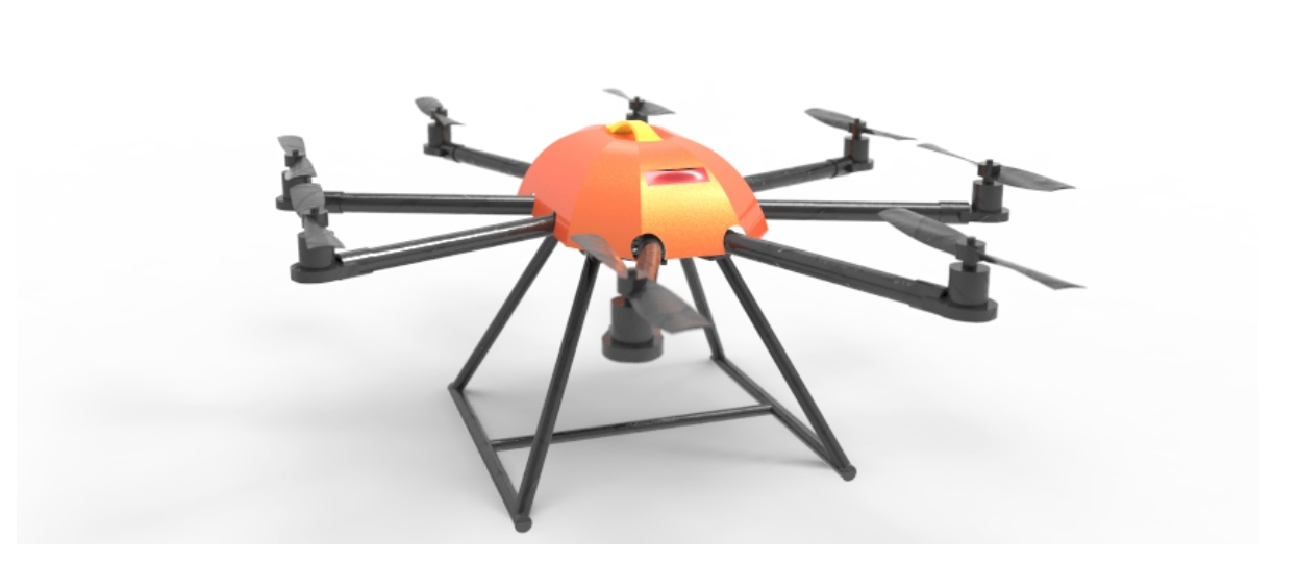
\includegraphics[keepaspectratio=true,scale=0.5]{figuras/keyshot1.eps}
    \caption{ Renderização do Projeto EmerVANT}
    \label{fig:keyshot1}
\end{figure}

O retângulo vermelho, na carcaça do EmerVANT, é a gaveta para retirada dos eletrodos do Desfibrilador Externo Automático, na qual o será orientado para o leigo, pela central, onde se encontra o eletrodos, juntamente todos os procedimentos de atendimento.

\begin{figure}[h!]
    \centering
      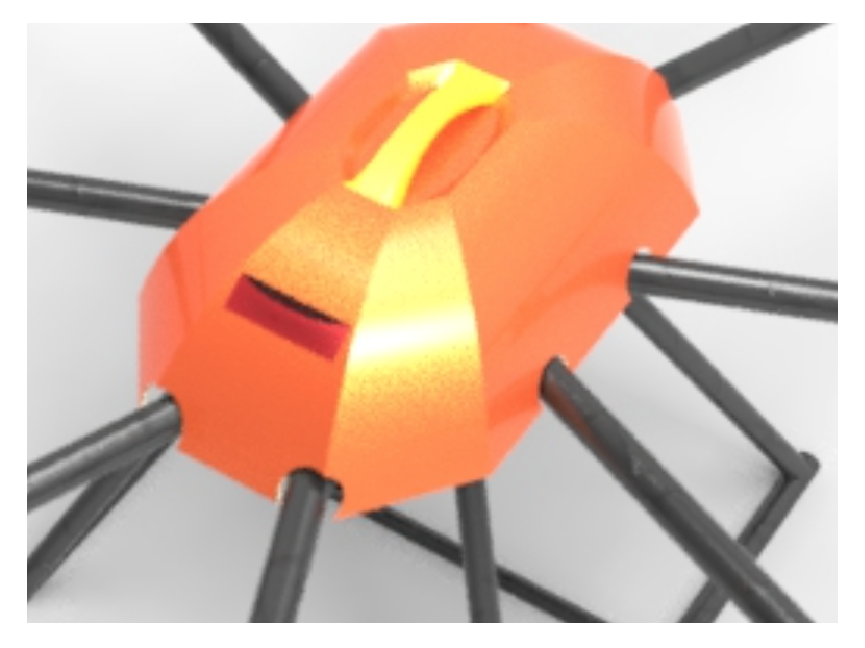
\includegraphics[keepaspectratio=true,scale=0.5]{figuras/keyshot2.eps}
    \caption{ Gaveta para eletrodos}
    \label{fig:keyshot2}
\end{figure}





















